\documentclass[table]{beamer}
%\usepackage[table]{xcolor}
\usepackage{amsmath, amsfonts, epsfig, xspace}
\usepackage[utf8]{inputenc}
\usepackage{algorithm,algorithmic}
\usepackage[normal,tight,center]{subfigure}
\setlength{\subfigcapskip}{-.5em}
\usepackage{beamerthemesplit}
% \usetheme{lankton-keynote}
\setbeamertemplate{headline}{} %Hide section stuff
\usepackage{natbib} %schönere Zitate
\usepackage{color}
\usepackage{fixltx2e}

\definecolor{OliveGreen}{RGB}{0,155,85}

\author{Jonathan Oberländer}

\title[Automatic Detection of LQ Violations\hspace{8em}\insertframenumber]{Automatic Detection of Linguistic Quality Violations} %\insertframenumber/\inserttotalframenumber

\date{}

\institute{Bachelor Thesis Defense\\Universität des Saarlandes\\21.08.2014}

\begin{document}

\maketitle

\section{Automatic Summarization}

\begin{frame}
  \frametitle{Automatic Summarization}
  \quad \quad 
\includegraphics[scale=0.1]{pics/documents.png} 
\includegraphics[scale=1]{pics/arrowlr.png} 
\includegraphics[scale=0.1]{pics/document.png}
\end{frame}

\begin{frame}
  \frametitle{Automatic Summarization}
  %types
  \begin{itemize}
    \item \textbf{Single-Document:} One document
    \item \textbf{Multi-Document:} Multiple documents on the same topic
  \end{itemize}
  \pause
  \begin{itemize}
    \item \textbf{Abstractive:} Internal semantic representation + generation
    \item \textbf{Extractive:} New summary from source sentences
  \end{itemize}
  \pause
  \vspace{1cm}

  \quad \quad \quad \begin{tabular}{r|c|c|}
    & Single-document & Multi-document\\
    \hline
    Abstractive & \cellcolor{red!25} & \cellcolor{red!25}\\
    \hline
    Extractive & \cellcolor{red!25} & \cellcolor{green!25}\\
    \hline
  \end{tabular}
  %…which hopefully produces coherent, grammatical sentences.
\end{frame}

\begin{frame}
  \frametitle{Linguistic Quality Violations}
  \textbf{Summarization systems \only<2->{\textcolor{red}{don't}}\only<1>{should} produce coherent and grammatical output.}
  \pause

  \textbf{Why?}
  \begin{itemize}
    \item It's hard.\pause
    \item Evaluation: content, information density
  \end{itemize}
  \vspace{1cm}
  \pause
  $\Rightarrow$ LQVCorpus \citep{friedrichlqvsumm}

  %doesn't always work. Why?

\end{frame}

\begin{frame}
  \frametitle{LQVCorpus \citep{friedrichlqvsumm}}
  %eckdaten, was wurde annotiert
  Annotated results of TAC 2011 Guided Summarization task \citep{owczarzak2011overview}
\pause
  \begin{itemize}
    \item Entity level:
    \begin{itemize}
      \item FM-EXPL, SM+EXPL%first mention without explanation%subsequent mention with explanation
      \item DNP-REF, INP+REF%definite noun phrase without reference to previous mention%indefinite noun phrase with reference to previous mention
      \item PRN-ANT, PRN+MISLA%pronoun with missing antecedent%pronoun with misleading antecedent
      \item ACR-EXPL%acronyms without explanations
    \end{itemize}\pause
    \item Clause level:
    \begin{itemize}
      \item \textbf{incomplete sentence (INCOMPLSN)}
      \item \textbf{inclusion of datelines (INCLDATE)}
      \item \textbf{other ungrammatical form (OTHRUNGR)}
      \item no semantic relatedness (NOSEMREL)
      \item \textbf{redundant information (REDUNINF)}
      \item no discourse relation (NODISREL)
    \end{itemize}
  \end{itemize}
\end{frame}

\begin{frame}
  \frametitle{Ungrammaticality (OTHRUNGR+INCOMPLSN)}
  %Many subtypes of ungrammaticality
  % \begin{itemize}
  %   \item Corpus study: actually many different types of violations
  % \end{itemize}
  \begin{center}
    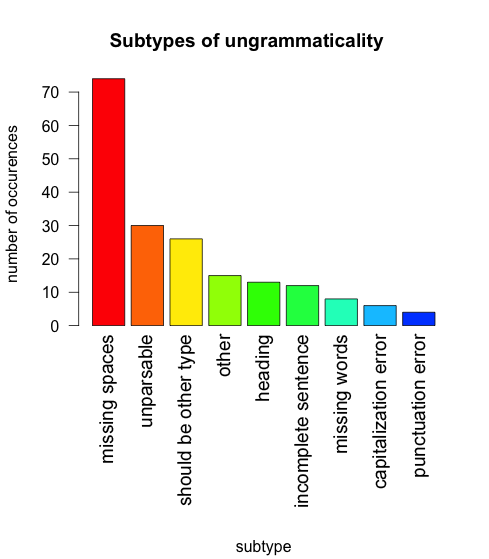
\includegraphics[scale=0.4]{subtypes_dev2.png}
  \end{center}
\end{frame}

\begin{frame}
  \frametitle{Detecting missing spaces}
  \textit{``A strong earthquake measuring 7.8 magnitude struck \textbf{Wenchuancounty} of Sichuan Province on Monday, leaving at least \textbf{12,000people} died and thousands more injured.''}

  \vspace{0.5cm}
  \textit{``Virginia Tech reported a campus shooting Monday and told \textbf{studentsto} stay inside their residences and away from windows.''}

  \vspace{0.5cm}
  \textit{``A gunman opened fire on classrooms at Virginia Tech University \textbf{onMonday} morning, killing at least 30 people before turning his \textbf{gunon} himself in the bloodiest school shooting in US history.''}
\end{frame}

\begin{frame}
  \frametitle{\textbf{UnknownTokens}}
  \textbf{Idea:}

  Sentence contains violation iff any word $\not\in$ known tokens
  \pause
  \vspace{0.6cm}

  \textbf{known tokens?}
  \begin{itemize}
    \item Source documents available? $\rightarrow$ all tokens in source documents = \textbf{UnknownTokens\textsubscript{source}}
    \item Otherwise $\rightarrow$ \textbf{UnknownTokens\textsubscript{general}}
  \end{itemize}
\end{frame}

\begin{frame}
  \frametitle{\textbf{UnknownTokens\textsubscript{general}}}
  \begin{itemize}
    \item Tokens from (parts of) Gigaword = \textbf{UnknownTokens\textsubscript{gw}}\pause
    \item + Heuristics (Capitalized words) = \textbf{UnknownTokens\textsubscript{gw+heur}}\pause
    \item + NER \citep{stanfordNER} = \textbf{UnknownTokens\textsubscript{gw+heur+ner}}\pause
    \item + Wikipedia = \textbf{UnknownTokens\textsubscript{gw+heur+ner+wiki}}
  \end{itemize}
\end{frame}

\begin{frame}
  \frametitle{\textbf{UnknownTokens}: Evaluation}
  \begin{tabular}{r|c|c|c|c|c|c|c|c|}
  & \multicolumn{3}{c|}{Missing spaces} & \multicolumn{3}{c|}{No missing spaces}\\
  & \textbf{P} & \textbf{R} & \textbf{F} & \textbf{P} & \textbf{R} & \textbf{F}\\
  \hline
  \textbf{Baseline} & 0.0 & 0.0 & 0.0 & 94.8 & \textbf{100} & 97.3\\
  \hline
  \textbf{UT\textsubscript{gw}} & 15.0 & \textbf{98.7} & 26.0 & \textbf{99.9} & 69.1 & 81.7\\
  \hline
  \textbf{UT\textsubscript{gw+heur}} & 30.5 & 97.3 & 46.5 & 99.8 & 87.8 & 93.4\\
  \hline
  \textbf{UT\textsubscript{gw+heur+ner}} & 35.5 & 97.3 & 52.0 & 99.8 & 90.3 & 94.8\\
  \hline
  \textbf{UT\textsubscript{gw+heur+ner+wiki}} & 70.3 & 96.0 & 81.2 & 99.8 & 97.8 & 98.8\\
  \hline
  \textbf{UT\textsubscript{source}} & \textbf{95.9} & 94.6 & \textbf{95.2} & 99.7 & 99.7 & \textbf{99.7}\\
  \hline
  \end{tabular}
\end{frame}

\begin{frame}
  \frametitle{\textbf{RandomForest}}
  RandomForest \citep{breiman2001random} to train decision trees
  \vspace{0.6cm}

  \textbf{Features:}
  \begin{itemize}
    \item classification from \textbf{UnknownTokens}\pause
    \item perplexity scores from language model trained on Gigaword\pause
    \item number of words
  \end{itemize}
\end{frame}

\begin{frame}
  \frametitle{\textbf{RandomForest}: Evaluation}
  \quad\quad\begin{tabular}{r|c|c|c|}
  & \textbf{Precision} & \textbf{Recall} & \textbf{F-Score}\\
  \hline
  Ungrammatical & 59.6 & 29.3 & 39.3\\
  \hline
  Not ungrammatical & 90.1 & 97.0 & 93.4\\
  \hline
  Weighted Average & 86.1 & 88.1 & 86.3\\
  \hline
  \end{tabular}
\end{frame}

\begin{frame}
  \frametitle{Datelines (INCLDATE)}
  \textit{\textbf{BLACKSBURG, Virginia 2007-04-16 18:34: 44 UTC} A gunman opened fire in a dorm and classroom at Virginia Tech on Monday, killing at least 30 people in the deadliest shooting rampage in U.S. history.}
  \vspace{0.5cm}

  \textit{\textbf{BERLIN, May 13( Xinhua)} The German government announced on Tuesday that it is to provide 500, 000 euros( around 770, 000 U.S. dollars) in aid for earthquake victims in Sichuan Province of China.}
  \vspace{0.5cm}

  \textit{\textbf{00 a.m.}People are panicking.}
\end{frame}

\begin{frame}
  \frametitle{Detecting Datelines}
  Regular expression:

  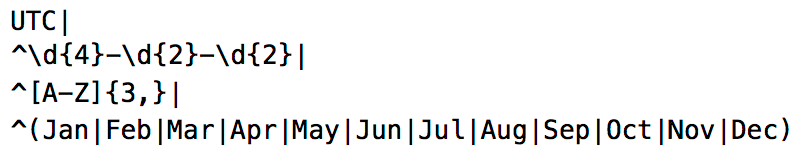
\includegraphics[scale=0.4]{regex.png}

  \vspace{1cm}\pause

  \begin{tabular}{|c|c|c|}
  \hline
  \textbf{Precision} & \textbf{Recall} & \textbf{F-Score}\\
  \hline
  90.3\% & 91.1 \% & 90.7\%\\
  \hline
  \end{tabular}
\end{frame}

\begin{frame}
  \frametitle{Redundancy (REDUNINF)}
  \textit{According to a survey by the State Food and Drug Administration, 65 percent of the respondents worried about the food safety situation in China. Food and drug safety has become a major concern of Chinese people.}
  \vspace{0.5cm}

  \textit{Cyclone Sidr, described as the worst storm in years to hit low-lying and disaster-prone Bangladesh, crashed into the southwestern coast Thursday night before sweeping north over the capital Dhaka. The cyclone hit the southwestern coast of Bangladesh on Thursday before sweeping north to the capital Dhaka.}
\end{frame}

\begin{frame}
  \frametitle{\textbf{Unigrams}}
  \begin{itemize}
    \item Remove non-alphanumeric characters and split into set of words\pause
    \item Cardinality of intersection between sets\pause
    \item Normalize by sentence length\pause
    \item Classify with threshold\pause
  \end{itemize}

  Variations: \textbf{Bigrams}, \textbf{Combined}

  \vspace{0.5cm}
  Threshold?
\end{frame}

\begin{frame}
  \frametitle{Finding a threshold}
  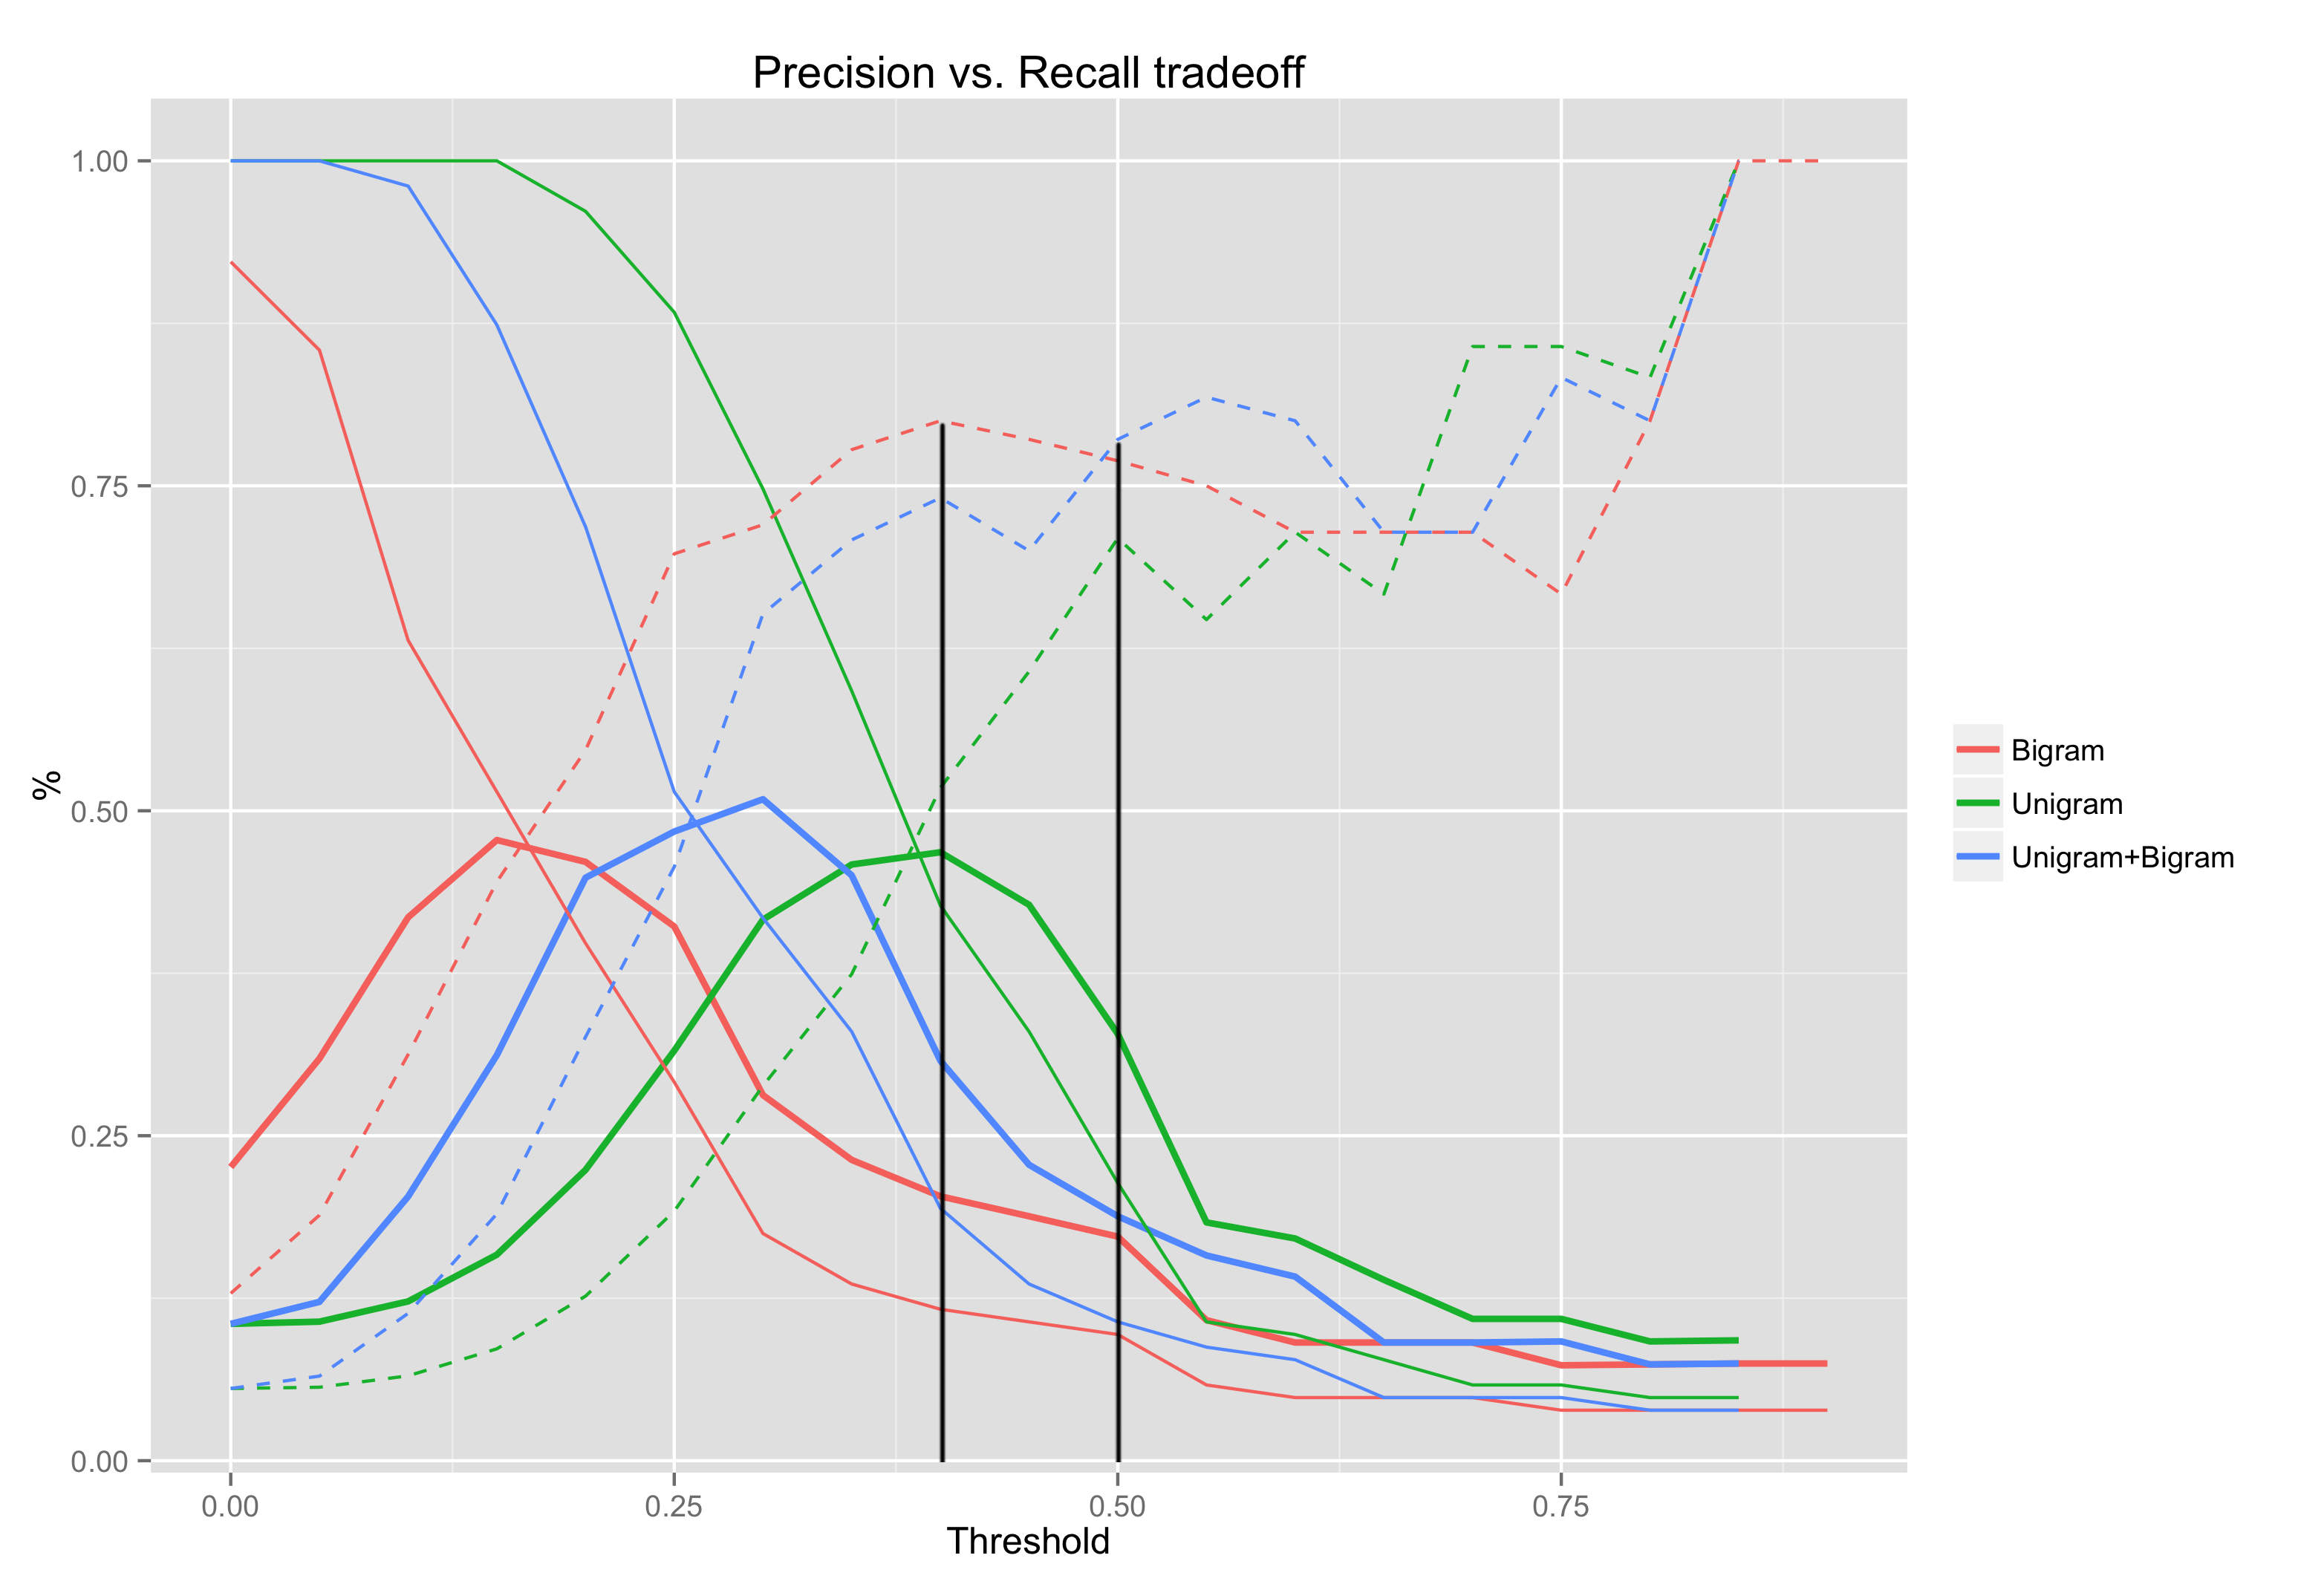
\includegraphics[scale=0.1]{a.png}
\end{frame}

\begin{frame}
  \frametitle{Evaluation of \textbf{Unigrams}, ...}
  \begin{tabular}{r|c|c|c|}
    & \textbf{Unigrams} & \textbf{Bigrams} & \textbf{Combined}\\
  \hline
  Threshold & 0.5 & 0.4 & 0.4
  \end{tabular}
  \vspace{1cm}

  \begin{tabular}{r|c|c|c|}
  & Precision & Recall & F-Score \\
  \hline
  \textbf{Baseline} & 4.5\% & \textbf{100\%} & 8.7\% \\
  \hline
  \textbf{Levenshtein} & 15.8\% & 17.3\% & 3.1\% \\
  \hline
  \textbf{Unigrams} & \textbf{58.0\%} & 28.2\% & \textbf{37.0\%} \\
  \hline
  \textbf{Bigrams} & 55.6\% & 14.5\% & 22.9\% \\
  \hline
  \textbf{Combined} & 56.8\% & 24.3\% & 34.0\% \\
  \hline
  \end{tabular}
\end{frame}

\begin{frame}
  \frametitle{References}
  \bibliographystyle{apalike}
  \bibliography{referenzen}
\end{frame}
\end{document}